\documentclass[10pt,journal,a4paper]{IEEEtran}

\usepackage{color}
\usepackage{overpic}
\usepackage{amssymb}
\usepackage{graphicx}
\usepackage{epstopdf}
\usepackage{amsmath}
\usepackage{graphicx}
\usepackage{amsfonts}
\usepackage{enumitem}
\usepackage{cite}
\usepackage{multirow}
\setlength{\parindent}{0pt}
\definecolor{mygray}{gray}{0.6}


\title{Convolution surfaces model  for hand tracking}

%\author{Anastasia Tkach\\ 
%Computer Graphics and Geometry Laboratory}

\begin{document}
\maketitle

\section{Introduction}

Hand tracking is a process of accurately reconstructing shape and articulation of human hands. It is a crucial component of natural human-computer interfaces and animation of humanoid avatars. A number of hand tracking algorithms has been recently proposed  Keskin et. al. \cite{keskin2012hand}, Melax et. al. \cite{melax2013dynamics}, Tang et. al. \cite{tang2013real}, Oikonomidis et. al. \cite{oikonomidis2014evolutionary}, Schroder et. al. \cite{schroder2014real},
Tompson et. al. \cite{tompson2014real}, Qian et. al. \cite{qian2014realtime},  Tagliasacchi et. al. \cite{tagliasacchi2015robust}, Sridhar et. al. \cite{sridhar2015fast}, Sun et. al. \cite{sun2015cascaded} and Sharp et. al. \cite{sharp2015accurate}.
However, in most consumer applications hand tracking is just a single components of a bigger pipeline (Figure \ref{fig:generic_pipeline}). Before tracking, a suitable hand model is obtained. Once the hand pose parameters are found, the tracking result is displayed by skinning the model. Both modeling and skinning tasks are not trivial.

\begin{figure}[h!] 
	\centering
	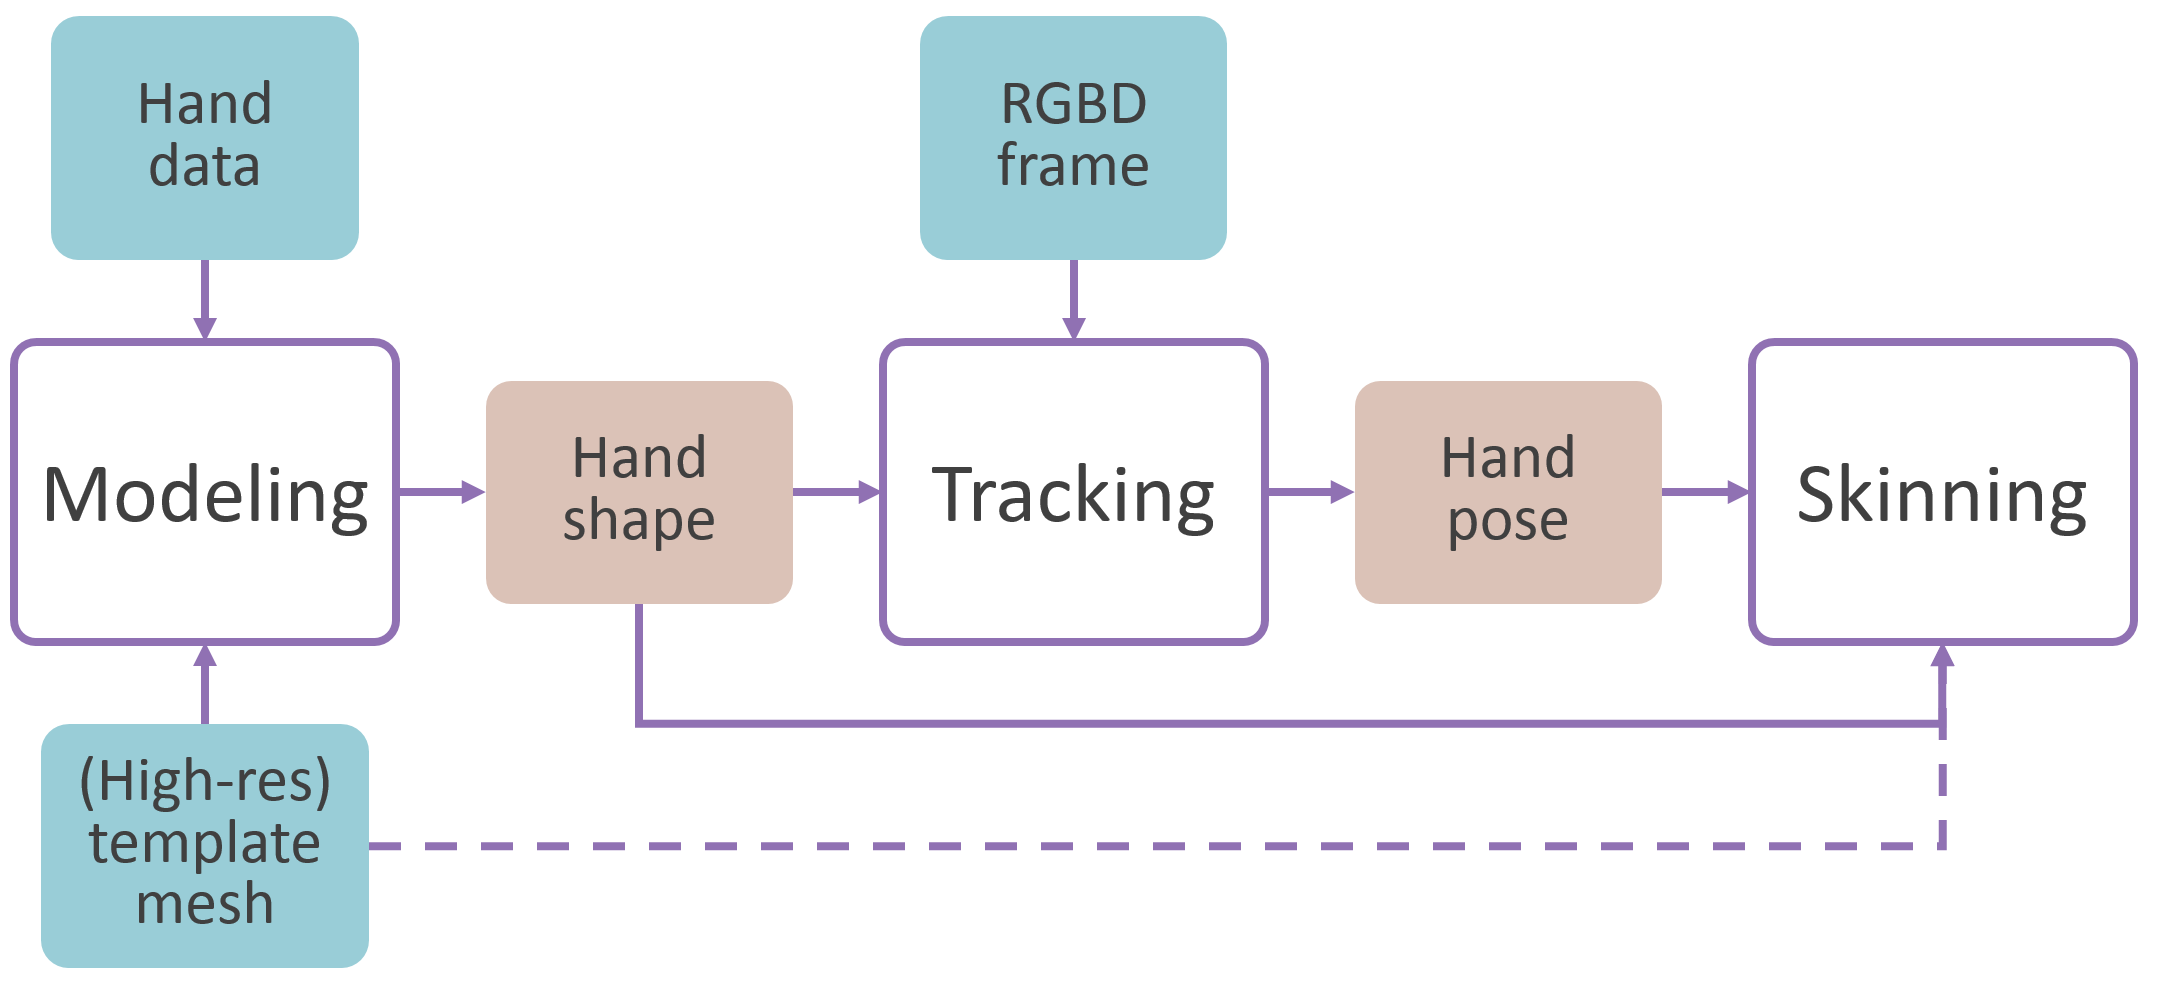
\includegraphics[width=0.5\textwidth]{figures/generic_pipeline}
	\caption{Generic pipeline for hand tracking. The input data that does not depend on the internal hand model representation is shown in blue, the representation-dependent components are shown in beige, and are listed in Table \ref{table:representation_dependent_components} for different representations.}
	\label{fig:generic_pipeline}
\end{figure}


\subsection{Why customizing the hand model?}

Hand model should be able to accurately represent the observed data.  The discrepancy between the optimal model pose given the data and the true hand pose can be significant, especially if the hand model does not reflect all the degrees of freedom of a hand (Figure \ref{fig:coarse_hand_model_and_lbs}, left).


\begin{figure}[h!] 
	\centering
	\hspace{-2em}
	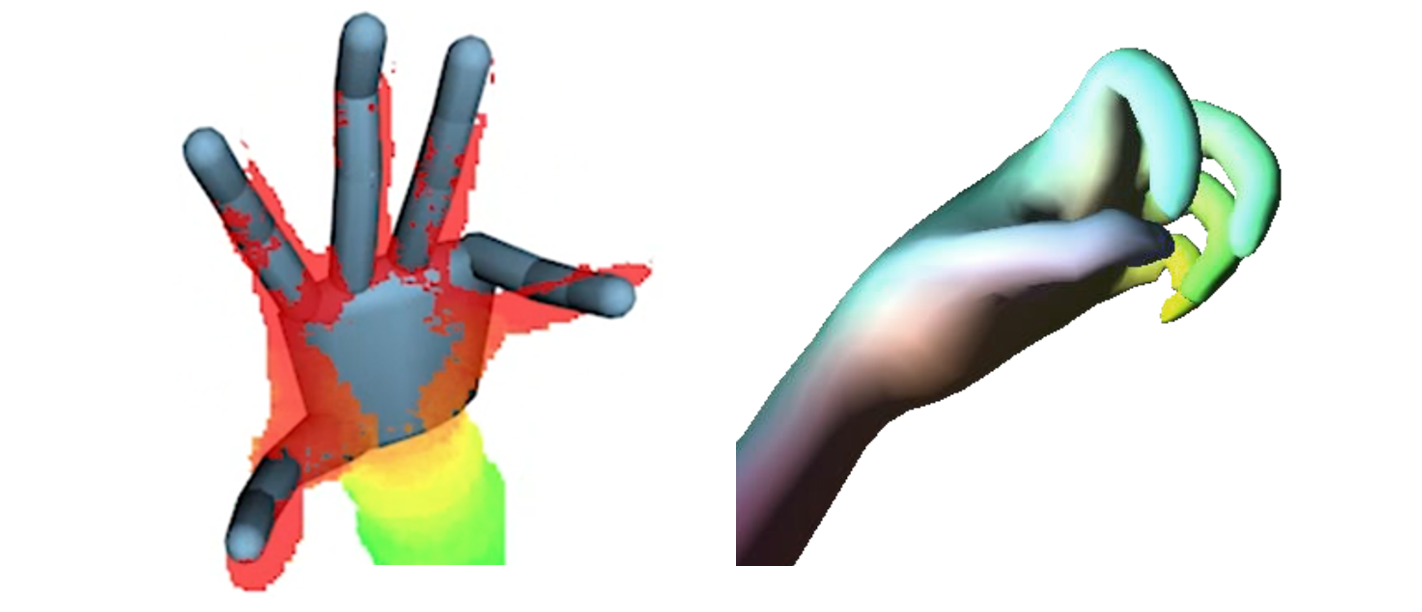
\includegraphics[width=0.5\textwidth]{figures/coarse_hand_model_and_lbs}
	\caption{Left - coarse hand model  from \cite{tagliasacchi2015robust}; right - hand model animated with linear blend skinning from \cite{sharp2015accurate}.}
	\label{fig:coarse_hand_model_and_lbs}
\end{figure}


\subsection{Why realistically animating the hand model?}

The hand skinning quality is obviously important for digital avatars applications. In AR and VR applications a 3D hand model can properly interact with 3D objects, establish a realistic contact and disappear behind them. Given that, the degree of immersion into virtual reality depends on whether a user sees own realistic hands \textcolor{mygray}{(find a study mentioned by Leap Motion).} The simple skinning approaches like linear blend skinning may generate implausible results  (Figure \ref{fig:coarse_hand_model_and_lbs}, right).

\subsection{Alternative hand model representations}
Each stage of the pipeline requires a hand model. There is several different hand model representations suggested by previous authors (see Figure \ref{fig:hand_model_representations}). Each representation is well suited for one of the stages, since it was used for the task on the first place. We argue that each representation also has weaknesses, which is why there exists a set of alternatives.

We suggest to use convolution surfaces representation of the hand model. 

Convolution surface is an implicit surface which is described by a control skeleton. The skeleton may consist of points, edges or polygons \cite{bloomenthal1991convolution}. In each vertex of the skeleton we define a radius. The radius in intermediate points is a linear combination of the radii at the neighboring vertices. Given the topology of the underlying skeleton, the model can be represented with convolution surface up to high precision \textcolor{mygray}{(find some theoretical estimates).} Next we present the arguments why convolution surfaces representation is suitable for all the stages of the pipeline.

\begin{table}[!h] 
	\centering
	\begin{tabular}{|p{2.5cm}|p{2.5cm}|p{2.5cm}|}
	\hline
 	& Hand pose  & Hand shape  \\
	\hline
	Triangular mesh with embedded skeleton, \cite{taylor2014user} & Vertices and bones positions & Vertices and bones positions	 \\
	\hline
	Cylinder model, \cite{tagliasacchi2015robust} & Cylinders size and transformations & Cylinders transformations	 \\
	\hline
	Convolution surfaces model & Positions and radii of control points & Positions of control points \\
	\hline
	\end{tabular}
	\vspace{1em}
	\caption{Comparison of different hand model representations}
	\label{table:representation_dependent_components}
\end{table}


\subsection{Convolution surfaces for model fitting}
The spheres and mixed cylinders/spheres hand model representations (Figure \ref{fig:hand_model_representations} a, b) are ubiquitous in hand tracking, because they are well suited for tracking tack per se (see next) and can be quickly to created manually. If a small number of  building blocks is used, the precision of the model is low, especially in the palm region. A higher precision can be obtained by increasing the number of primitives, which defeats the purpose of model simplicity. Convolution surfaces representation gives higher precision for the same number of building blocks. \textcolor{mygray}{Add experimental or theoretical support for convolution surfaces.}
The triangles mesh representation can approximate the hand to a high precision. However, there is obvious way to specify the model parts that are rigid and should be kept the same shape between the poses. This results in overfitting to local skin deformations. 

\begin{figure}[h!] 
	\centering
	\hspace{-2em}
	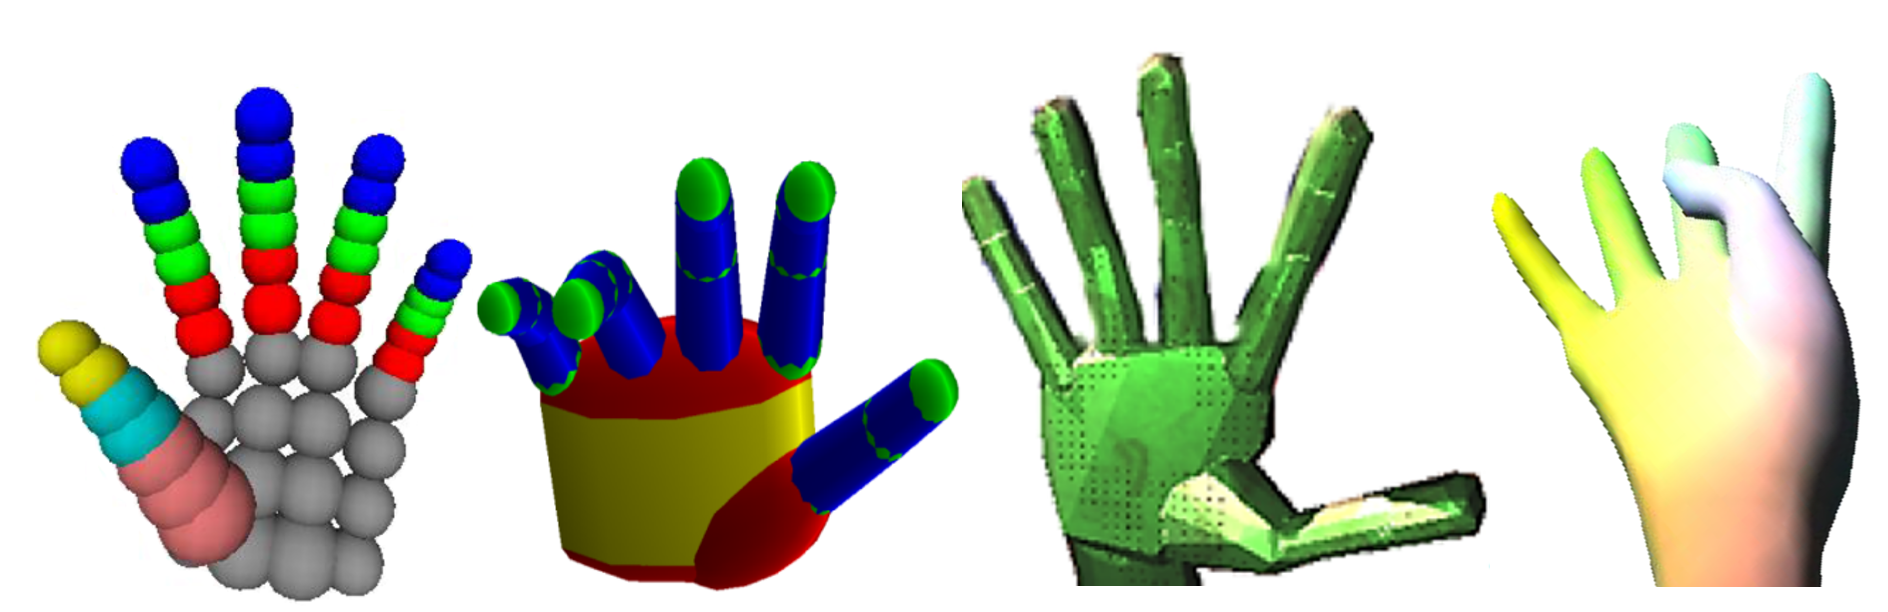
\includegraphics[width=0.5\textwidth]{figures/hand_model_representations}
	\caption{Hand model representations from works of (a) Qian et. al. \cite{qian2014realtime}, (b)  Oikonomidis et. al. \cite{oikonomidis2014evolutionary}, (c) Melax et. al. \cite{melax2013dynamics} and (d) Sharp et. al \cite{sharp2015accurate}.}
	\label{fig:hand_model_representations}
\end{figure}

\subsection{Convolution surfaces for hand tracking}
For model based tracking the main operation is to find the closest point on the model for a given data point. This operation is can be done in closed for each rigid segment with spheres/cylinder and convolution surfaces model representation. For a triangular mesh this operation has complexity linear in number of triangles. Moreover, the triangular mesh has (much) more degrees of freedom than the underlying problem. Without additional regularization, rigid parts of the hand model can deform to fit the data and the individual vertices can shift to fit the sensor noise.

\subsection{Convolution surfaces for hand skinning}
The Linear Blend Skinning approach used to pose the triangular mesh model in previous works (\cite{sharp2015accurate}, \cite{schroder2013analysis} ) creates artifacts, the fingers looks like made from rubber. The spheres/cylinders model is not suitable for realistic animation, therefore a re-targeting step to a template mesh is required. Retargeting does not only demand additional effort, but also brings additional imprecision. The state of the art approaches in hand skinning are implicit surfaces-based (\cite{vaillant2013implicit},  \cite{vaillant2014robust} ).  A convolution surfaces model serves a ready to use input for such an approach.

\subsection{Contributions}

\begin{itemize}

\item Developed an approach for approximation a model with convolution surface, given a skeleton topology.
\item Formulated position-based inverse kinematics algorithm for hand tracking. The position based approach does not require walking through the hierarchical chain of joint, thus saving the computational power. Also, position-based inverse kinematics does not involve linear approximations or rotations, thus making the optimization more stable.
\item Suggested an automatic approach for field functions construction in implicit skinning.  \textcolor{mygray}{Replaced newton iteration for vertex projection by a closed form solution.}

\end{itemize}


%%%%%%%%%%%%%%%%%%%%%%%%%%%%%%%%%%%%%%%%%%%%%%%%%%%%%%%%%%%%%%%%%%%%%%%%

\section{Related Literature}

\begin{itemize}

\item Albrecht et al. \cite{albrecht2003construction} developed an approach for creating an anatomically realistic hand model that includes bones and muscles structure. Their approach requires several prerequisites including plaster cast of a human hand and laser scanner for manually creating a physically realistic hand template. Given user-defined correspondences between 3D feature points and the hand image, a specific hand model is created by deforming a generic hand model. 

\item Rhee et. al. \cite{rhee2006human} use a single image of a hand at rest pose to infer joint hand joint locations from skin creases. Given the skeleton obtained at the previous step and the hand contour from the image, they deform a template hand mesh to fit this data. 

\item Straka et al. \cite{straka2012simultaneous} also fit the template mesh with attached skeleton to 3D data. The model is deformed to explain the data while keeping the vertices attached to their corresponding bones. It is on clear whether the approach whether be able to handle a hand motion sequence, since the results are demonstrated on a full body model.

\item Taylor et. al. \cite{taylor2014user} generate a user-specific hand model from an RGBD video sequence. The model is represented as a triangular mesh with an embedded skeleton. In each frame the hand pose is initialized using an appearance-based tracking algorithm. The hand model parameters are found by solving a single optimization problem formulated for the entire video sequence which also finds hand pose in each frame. 

\item Khamis et. al.  \cite{khamis12learning} fit a hand model for a specific user by finding its shape coordinates in the basis of mesh matrices and bones locations. As in the approach by Taylor et. al, they optimize simultaneously for pose and shape parameters in all the frames of an RGBD sequence across all the subjects. Requires large number of subjects as a regularization for excessive degrees of freedom. 

The results generated by the approaches listed above could be used as an input for our system to create a hand model representation adapted for efficient tracking and animation.


\end{itemize}


%%%%%%%%%%%%%%%%%%%%%%%%%%%%%%%%%%%%%%%%%%%%%%%%%%%%%%%%%%%%%%%%%%%%%%%%

\section{Results}

\subsection{Modeling}

\begin{figure}[h!] 
	\centering
	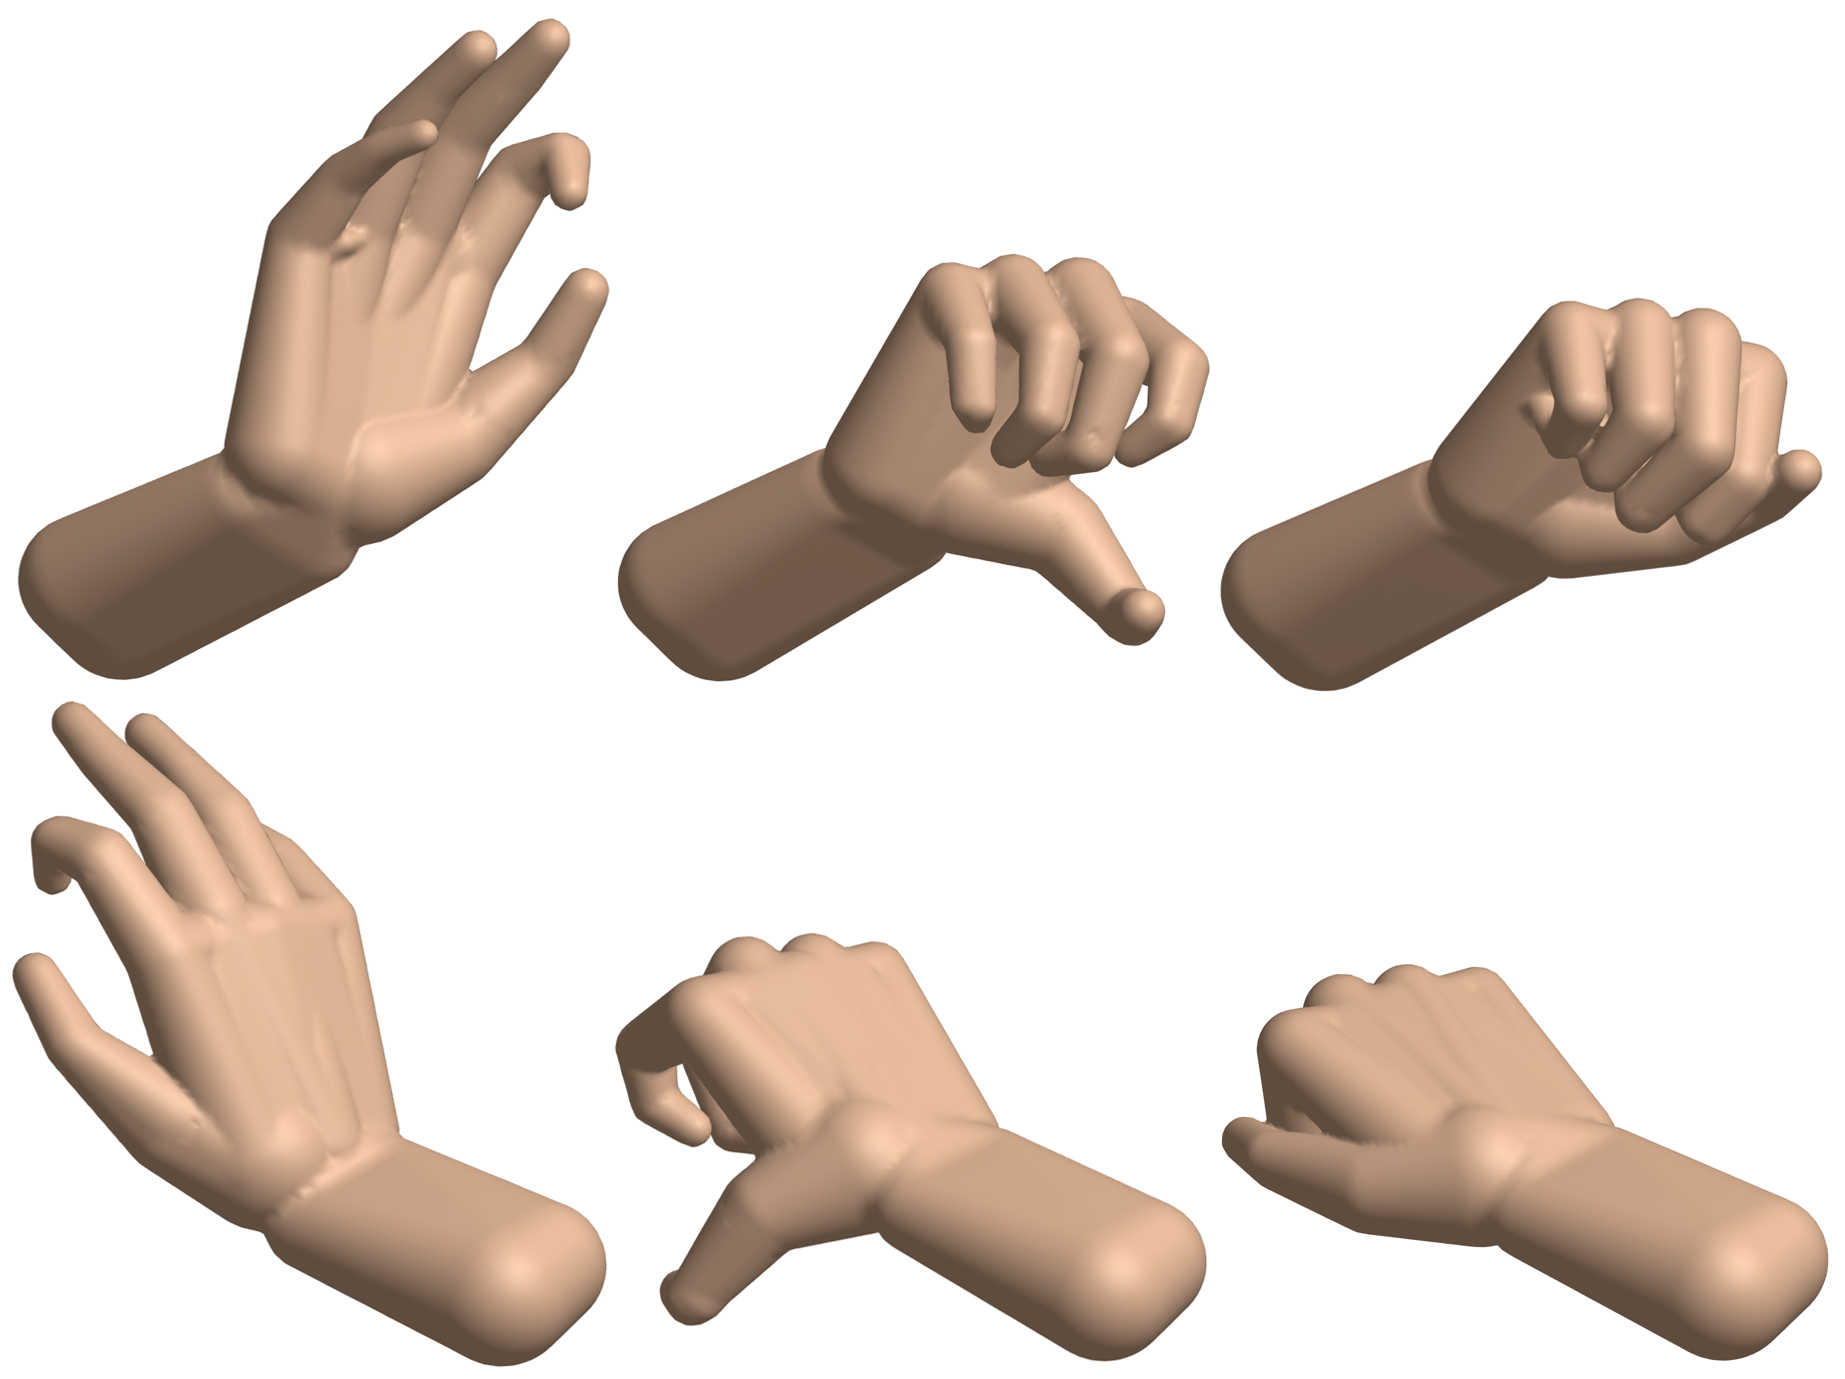
\includegraphics[width=0.5\textwidth]{figures/modeling}
	\caption{Fitting convolution surfaces hand model to several poses of the same hand.}
	\label{fig:modeling}
\end{figure}

\subsection{Tracking}

\subsection{Skinning}

%%%%%%%%%%%%%%%%%%%%%%%%%%%%%%%%%%%%%%%%%%%%%%%%%%%%%%%%%%%%%%%%%%%%%%%%

\appendix
\subsection{Convolution segment}

\begin{figure}[h!] 
	\centering
	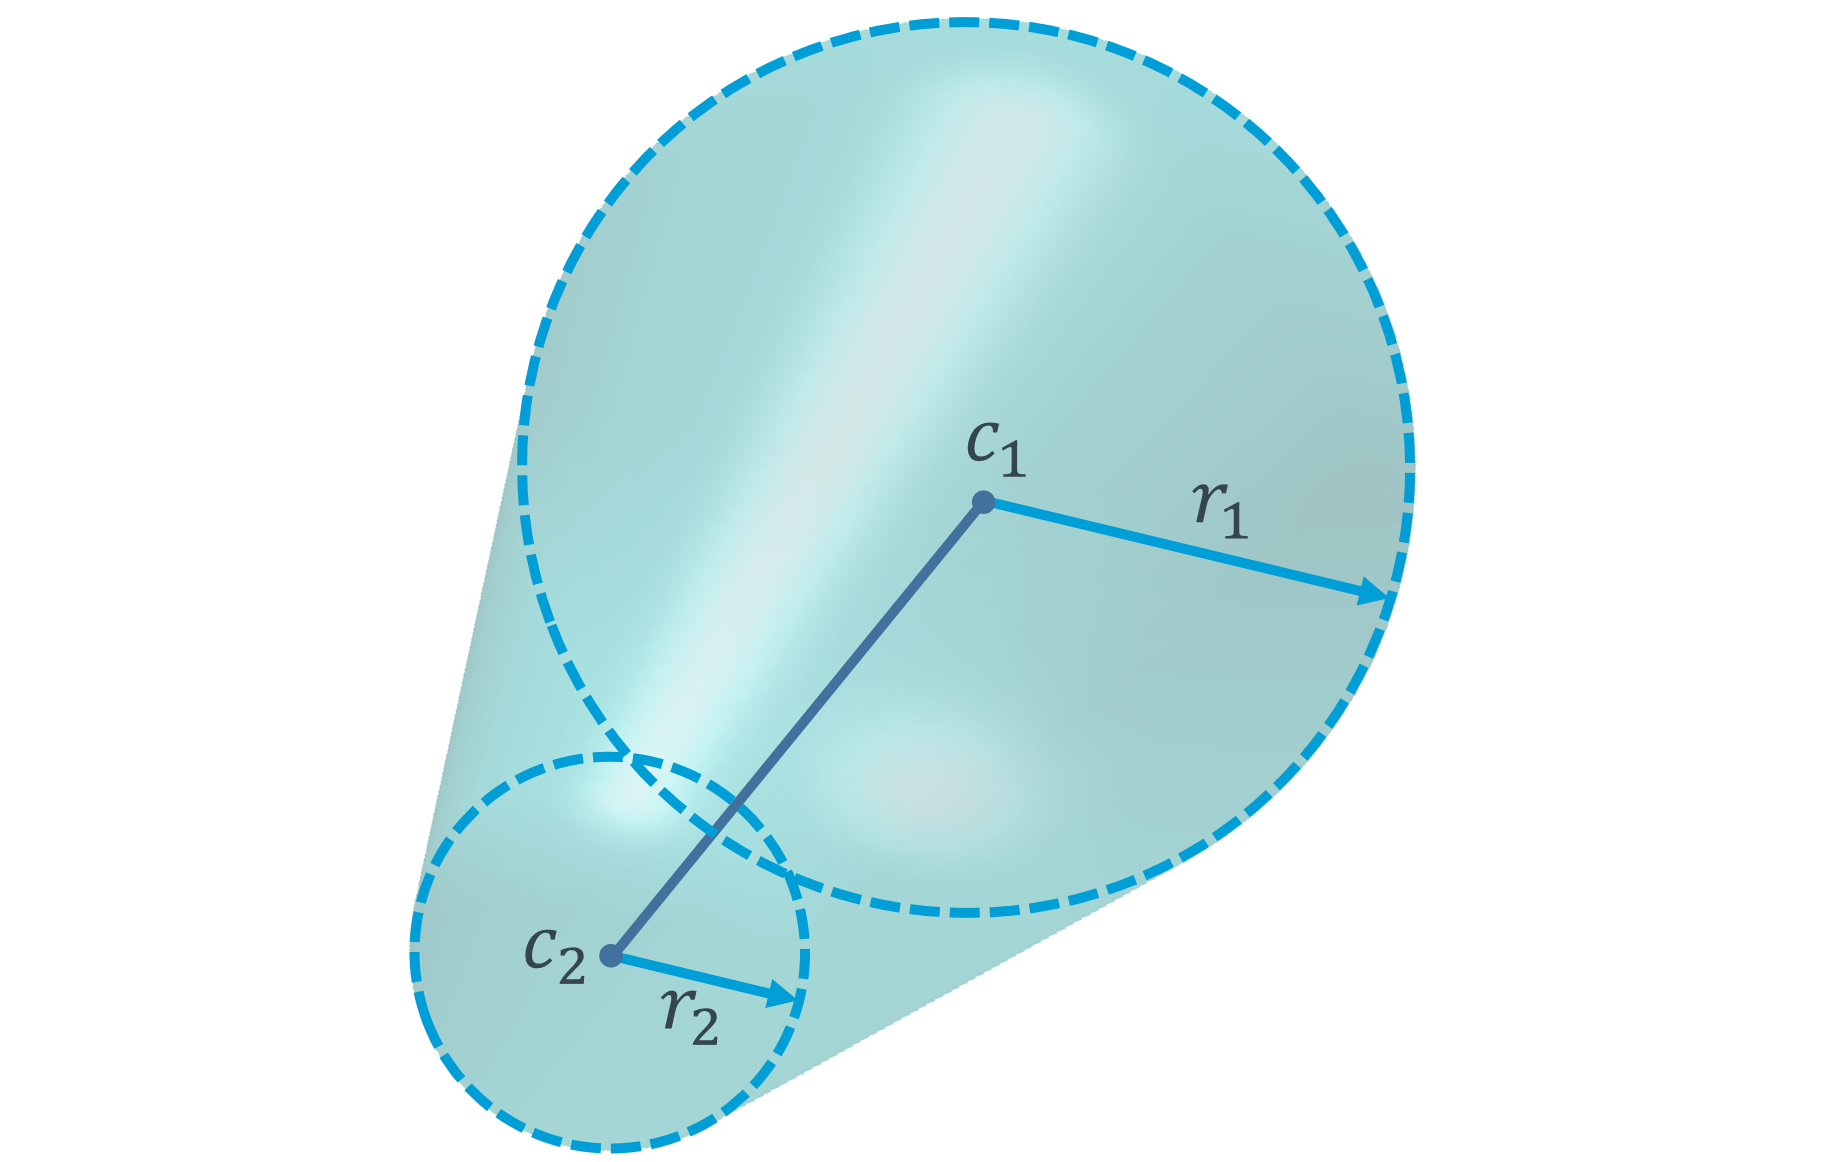
\includegraphics[width=0.5\textwidth]{figures/convsegment.png}
	\caption{Convolution segment.}
	\label{fig:convsegment}
\end{figure}

A convolution segment (Figure \ref{fig:convsegment}) is defined by two spheres $S_1 = \{c_1, r_1\}$ and $S_2 = \{c_2, r_2\}$.
Given the data points $P = \{p_i\}_{i = 1}^N$ and their projections on the model  $Q = \{q_i(c_1, c_2, r_1, r_2)\}_{i = 1}^N$  we construct a vector-function $\textbf{f}$ 

 \begin{equation}
 	\textbf{f} = \left[
 		\begin{array}{c}
 			\vdots \\
			p_i^x - q_i^x\\
			p_i^y - q_i^y\\
			p_i^z - q_i^z\\
			\vdots \\
	\end{array}
 	\right].
 \end{equation} 

\begin{figure}[h!] 
	\centering
	\hspace{-2em}
	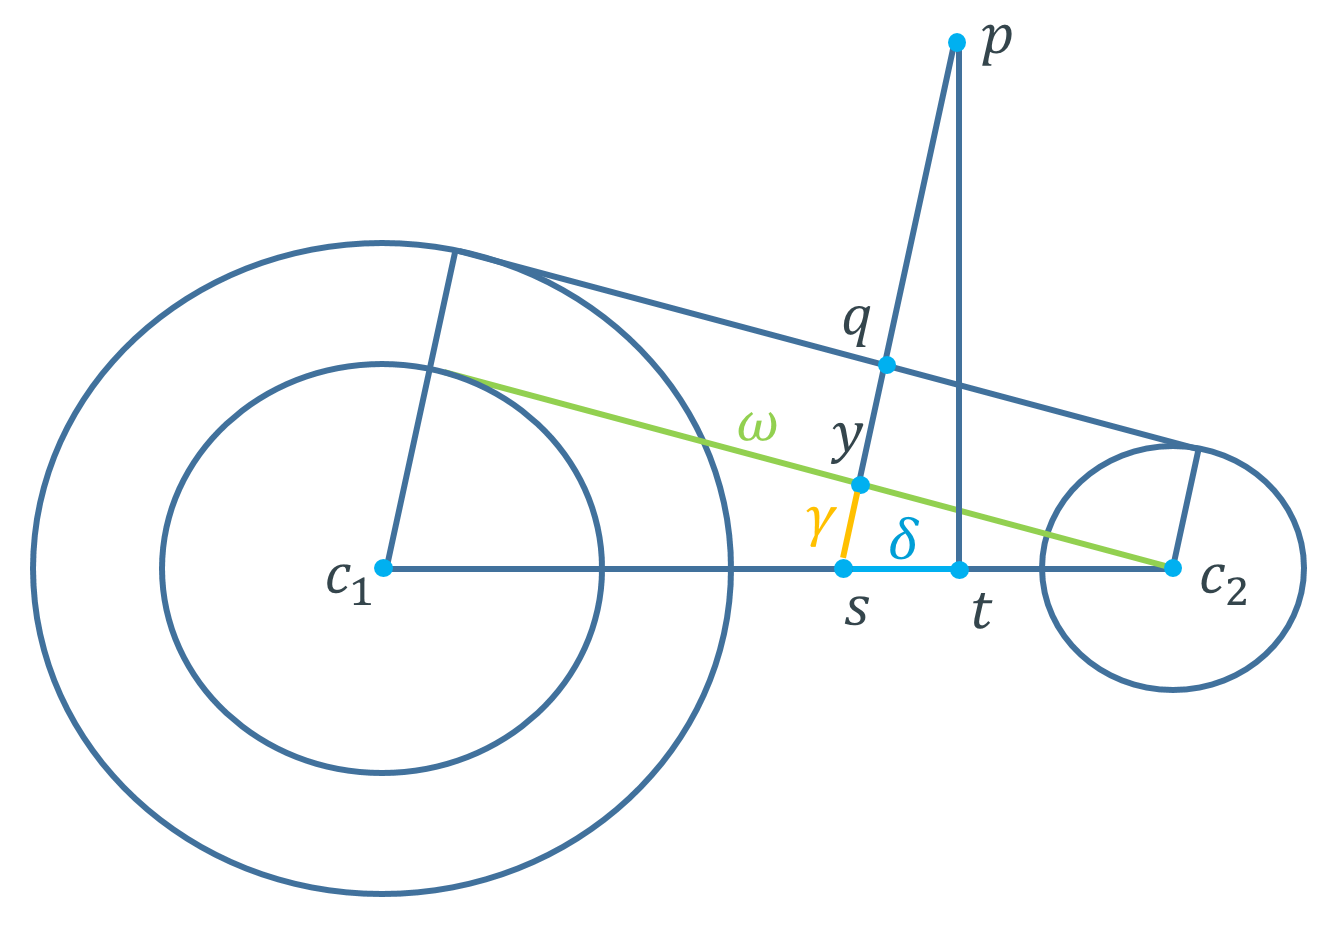
\includegraphics[width=0.47\textwidth]{figures/projection_convsegment.png}
	\caption{Convolution segment.}
	\label{fig:projection_convsegment}
\end{figure}

To fit the model to the data, we iteratively minimize $\textbf{f}$ using Levenberg-Marquardt iteration. In order to compute the Jacobian, the projections $q_i$ should be expressed as functions of model parameters. Let us first find the projection $q$ of a point $p$ on the segment $\{c_1, c_2\}$. Assume that $c_1 > c_2$. If the point on the segment $t$ closest to $p$ lies at the end of the segment, say, $c_1$, than $q = c_1 + \frac{r_1  (p - c_1)}{\Vert p - c_1 \Vert}$. 
Otherwise, the projection $q$ is computed as 

\begin{align*}
& u = c_2 - c_1, \\
& v = p - c_1, \\
& \omega = \sqrt{u^T u - (r_1 - r_2)^2}, \\
&  \delta =  \frac{(r_1 - r_2) \Vert p - t \Vert}{\omega}, \\
&   s = t - \delta  \frac{c_2 - c_1} {\Vert c_2 - c_1 \Vert}, \\
&  \gamma = \frac{(r_1 - r_2)   {\Vert c_2 - t + \delta  \frac{u} {\Vert u \Vert}} \Vert} {\Vert u \Vert}, \\
&   q = s +\frac{ (p - s) (\gamma + r_2) }{ \Vert p - s \Vert } .
\end{align*}

(See Figure \ref{fig:projection_convsegment}).

Given the projection $q_i = q_i(c_1, c_2, r_1, r_2)$, the objective function $\textbf{f} = [\cdots, f_i^T, \cdots]^T$  has the Jacobian $\textbf{J}$ with $J_{ij} = \frac{\partial{f_i}}{\partial{x_j}}$, where $\textbf{x} = [c_1, c_2, r_1, r_2]$.  At each iteration of Levenberg-Marquardt , we first compute the data-model correspondences. In case of convolution segments this amounts to determining whether the closest point is located at one of the end points of the segment or lies in between. Given this correspondence, the Jacobian is computed using chain rule, by composition of derivatives of algebraic operations required to find $q(c_1, c_2, r_1, r_2)$.


%%%%%%%%%%%%%%%%%%%%%%%%%%%%%%%%%%%%%%%%%%%%%%%%%%%%%%%%%%%%%%%%%%%%%%%%


\subsection{Convolution triangle}


\begin{figure}[h!] 
	\centering
	\hspace{-2em}
	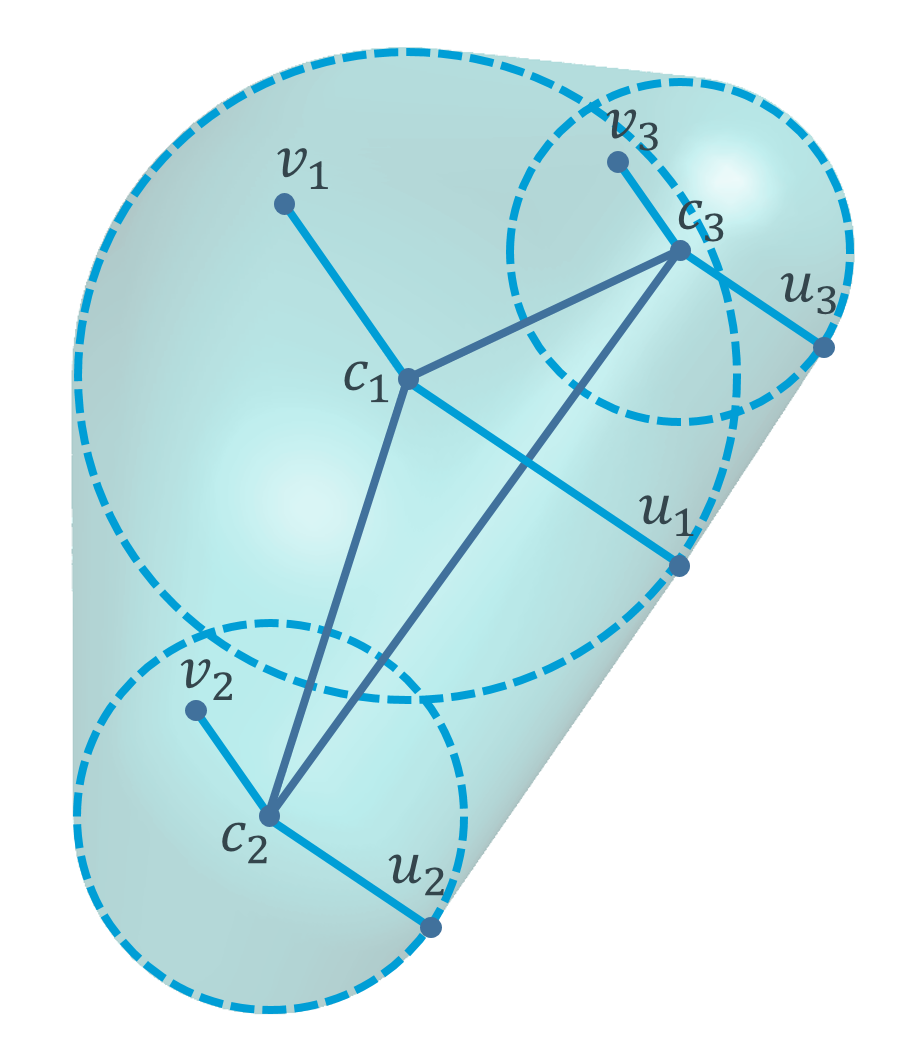
\includegraphics[width=0.3\textwidth]{figures/convtriangle.png}
	\caption{Convolution triangle.}
	\label{fig:convtriangle}
\end{figure}

A convolution triangle (Figure \ref{fig:convtriangle}) is defined by three spheres $S_1 = \{c_1, r_1\}$, $S_2 = \{c_2, r_2\}$ and $S_3 = \{c_3, r_3\}$. To express the projection $q_i$ as a function of the model parameters, first, let us find the outer tangent planes for the spheres. There exists two outer tangent planes if none of the spheres lies entirely inside of the cone tangent to the other two spheres. 

\begin{figure}[h!] 
	\centering
	\hspace{-2em}
	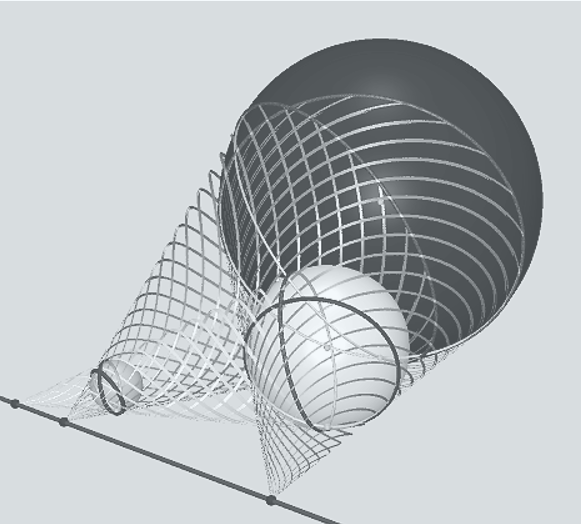
\includegraphics[width=0.45\textwidth]{figures/cones_and_tangent_plane.png}
	\caption{The three apices of the cones tangent to each pair of spheres lie on a straight line.}
	\label{fig:logistic_regression}
\end{figure}

\begin{figure}[h!] 
	\centering
	\hspace{-2em}
	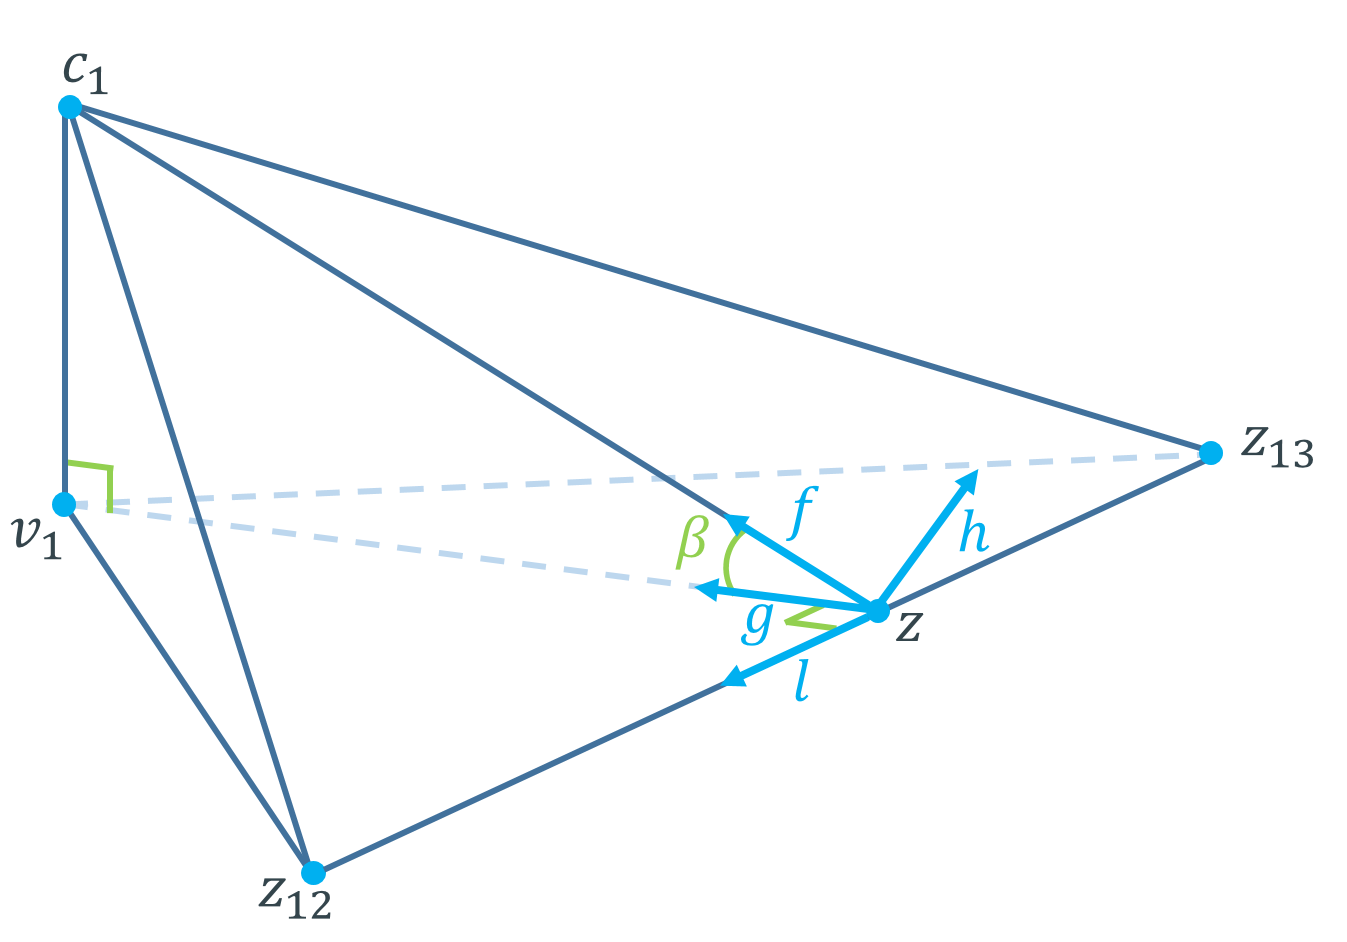
\includegraphics[width=0.45\textwidth]{figures/projection_convtriangle.png}
	\caption{Computing the tangent plane for three spheres.}
	\label{fig:projection_convtriangle}
\end{figure}

\subsection{Computing the tangent plane}

In Figure \ref{fig:projection_convtriangle}, the point $z_{12}$ is an apex of a cone tangent to the spheres $S_1$ and $S_2$. The position of $z_{12}$ can be found from similarity of triangles:

\begin{equation}
	z_{12} = c_1 +\frac{r_1 (c_2 - c_1)}{r_1 - r_2},
\end{equation}

In the same way,

\begin{equation}
	z_{13} = c_1 +\frac{r_1 (c_3 - c_1)}{r_1 - r_3}.
\end{equation}

The direction vector $l$ of the line, that contains the apices of the tangent cones is found as

\begin{equation}
	l = \frac{z_{12} - z_{13}} {\Vert z_{12} - z_{13} \Vert} 
\end{equation}

The intersection point of the plane orthogonal to $l$ and going through the point $c_1$ with the line going through $z_{12}$ and $z_{13}$ is found as

\begin{equation}
z = z_{12} + ((c_1 - z_{12})^T l )l.
\end{equation}

The sine and cosine of the angle $\beta$ in triangle $\{c_1, z, v_1\}$ are given by 

\begin{equation}
	\sin(\beta) = \frac{r_1}{\eta},
\end{equation}

\begin{equation}
	\cos(\beta) = \frac{\nu}{\eta},
\end{equation}

where $\eta = \Vert c_1 - z \Vert $ and $\nu = \sqrt{\eta^2 -  r_1^2}$. 

Denote the tangent point of the sphere $S_1$ as $v_1$. The direction vector $g$ of the line $\{c_1, v_1\}$ can be found by rotating the direction vector $f$ of the line 
$\{c_1, z\}$ by angle $\beta$ around the axis $l$.

\begin{align}
	& h = \frac{l \times f}{\Vert l \times f \Vert}, \\
	& g = \sin(\beta) h + \cos(\beta) f.	
\end{align}

The tangent point $v_1$ is found as
\begin{equation}
v_1 = z + \nu  g
\end{equation}


Having the normal vector of the tangent plane $n = \frac{v_1 - c_1}{\Vert v_1 - c_1 \Vert}$, we can find the tangent points of the spheres $S_2$ and $S_3$:

\begin{align}
	& v_2 = c_2  + r_2 n \\
	& v_3 = c_3 + r_3 n 
\end{align}

The second tangent plane $\{u_1, u_2, u_3$\} is found by rotating the vector $f$ around the axis $l$ by an angle $-\beta$.



\subsection{Computing the projection}

If the point, closest to $p$ on triangle $\{v_1, v_2, v_3\}$ or on triangle $\{u_1, u_2, u_3\}$ lies inside of the triangle, than it is the projection $q$. Otherwise $q$ belongs to the surface of one of the convolution segments $\{c_1, c_2\}$,  $\{c_1, c_3\}$, or  $\{c_1, c_3\}$. Thus, the candidates for $q$ are the projections of $p$ on the segments $q_{12}$, $q_{13}$ or $q_{23}$. The projection $q$ is determined taking into account the distance to $p$ and whether  $q_{12}$, $q_{13}$ and $q_{23}$ are located inside or outside of the segments $\{c_1, c_2\}$,  $\{c_1, c_3\}$, and  $\{c_1, c_3\}$.  

%%%%%%%%%%%%%%%%%%%%%%%%%%%%%%%%%%%%%%%%%%%%%%%%%%%%%%%%%%%%%%%%%%%%%%%%

\section{Combining several blocks}

Consider the case when several convolution segments and triangles are used to create a more complex model. To find the projection $q$, we compute a projection $q_j$ on each  building block.  The projection $q$ is determined taking into account the distances between $q_j$ and $p$ and whether  $q_j$ are located inside or outside of the building blocks.

%%%%%%%%%%%%%%%%%%%%%%%%%%%%%%%%%%%%%%%%%%%%%%%%%%%%%%%%%%%%%%%%%%%%%%%%


 \bibliographystyle{plain}
\bibliography{hmodel}

\end{document}
